
\chapter*{Einleitung}\thispagestyle{fancy}\markboth{Einleitung}{Einleitung}
\addcontentsline{toc}{chapter}{Einleitung}




In den letzten Jahren ist die Energieversorgung mit Hilfe von erneuerbaren Energieträgern wie Wind, Sonne und Biomasse immer weiter in den Vordergrund gerückt. Um die endlichen fossilen Ressourcen zu  schonen sind wir über kurz oder lang auf den Ausbau von regenerativen Energieerzeugern angewiesen. Mit dem Gesetz für den Ausbau erneuerbarer Energien welches am 01.08.2014 in Kraft getreten ist wurden von der Bundesregierung klare Regelungen zum zukünftigen Ausbau der erneuerbaren Energien verfasst. Dort wird festgelegt, dass der 
"` ... Anteil des an erneuerbaren Energien erzeugten Stroms am Bruttostromverbrauch auf mindestens 80 Prozent bis zum Jahr 2050 ..."'(\cite{Bundestag.21.07.2014}EEG 2014, §1Abs.2) zu erhöhen ist. Jedoch würde dieser Ausbau eine steigende Volatilität im Übertragungsnetz mit sich bringen. Im europäischen Verbundnetz ist die Netzfrequenz von 50Hz mit einer zulässigen, maximalen Abweichung von 0,2 Hz genormt. Bei einem Überangebot von produziertem Strom würde die Netzfrequenz ansteigen, sowie sie bei überhöhter Last (Stromentnahme durch Verbraucher) sinken würde. Um diese Schwankungen so ausgleichen zu können, dass die Netzfrequenz innerhalb der festgesetzten Toleranz bleibt, müssen Kraftwerke mit viel Aufwand, verbunden mit hohen Kosten, geregelt werden. Um nun also unvorhergesehene Lastschwankungen im Stromnetz ausgleichen zu können muss der ÜNB genügend Regelleistung vorhalten. Hierbei wird abhängig von Systemreaktionszeit und  möglicher Einsatzdauer in Primärregelenergie, Sekundärregelenergie und Minutenreserve unterschieden. 
\begin{figure}[h]
	\centering
		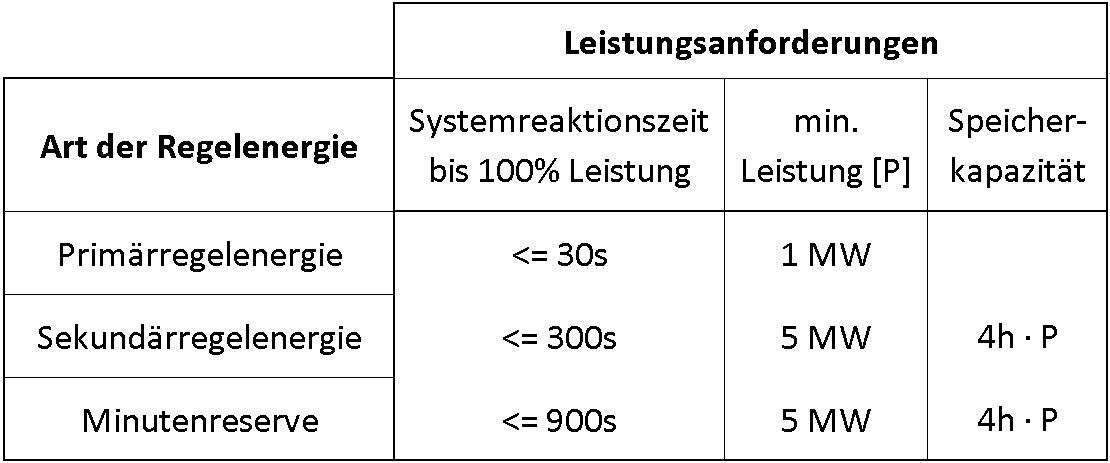
\includegraphics[width=0.90\textwidth]{images/Tabelle_Regelenergien.JPG}
	\caption{Anforderung an Regelenergien}
	\label{fig:Tabelle Regelenergien}
\end{figure}

Ein wichtiger Punkt hierbei sind Energiespeichersysteme, welche genau für diese Anwendungsfälle Regelleistung bereitstellen können. Speziell für kurzzeitige Ausregelungen von Lastspitzen oder Einspeisungseinbrüchen von PV-Anlagen oder auch für die Bereitstellung von Pri-märregelleistung in Übertragungsnetzen erweisen sich Batteriespeicher als durchaus geeignetes Mittel. Mit Hilfe dieser Batteriespeichertechnologien können durch spezielle Regelalgorythmen PV-Kraftwerke wesentlich gleichmäßiger Energie in das Übertragungsnetz einspeisen. Die Belectric GmbH hat mittlerweile marktreife Konzepte entwickelt um PV-Kraftwerke gekoppelt mit Batteriespeichern ( bezeichnet als Hybrid 1) oder auch PV-Kraftwerke gekoppelt mit Batteriespeichern und Dieselgeneratoren (bezeichnet als Hybrid 2) zu betreiben. Ein wesentlicher Vorteil dieser Hybridisierung von PV-Kraftwerken liegt darin, dass aufgrund der besseren Regelcharakteristik deutlich mehr Leistung installiert werden kann ohne die Übertragungsnetze zu überlasten, wodurch die Kosteneffizienz erheblich steigt.  



